\subsection{Design Goals}

We want to provide an architecture for web data processing that is based on unified treatment of data on annotation and processing side
and that allows the backend machinery to access all information contained in a web page, including how it is presented to a web surfer.

\subsection{Requirements}

\begin{description}

\item[Flexibility]
The system should be open enough to allow customization of every part, but also specifically provide stable interfaces for more common tasks to allow for modularization.

\item[Stability]
We need a stable http data source that is independent of the original website, including any dependencies such as images, stylesheets or scripts.

\item[Automaticity]
Backend processing should run without requiring any kind of human interaction.

\item[Replicability]
Computations carried out on web pages' representation must be replicable accross systems, including any user-side processing.

\item[Quantity]
Corpus size should not influence the performance of the system and total processing time should grow linearly with the corpus.

\item[Usability]
Usability of the annotators side is of paramount importance, so we should stay as close as possible to the everyday web experience.
We also need to provide tools for learning how to use the annotation tool and how to annotate web pages.

\end{description}

\subsection{Core Architecture}

The World Wide Web Consortium's DOM Standard \cite{dom} provides a unified for accessing attributes of a rendered web page.

\begin{figure}
\jss{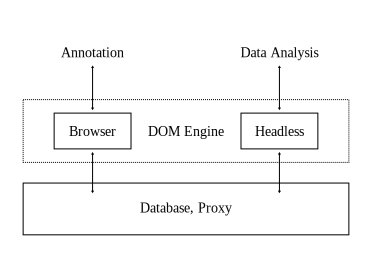
\includegraphics[width=0.5\textwidth]{arch}}
	{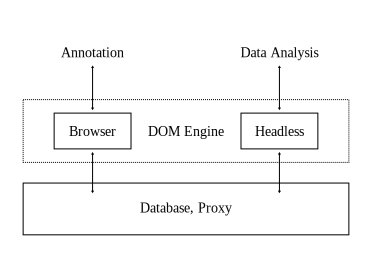
\includegraphics[width=\textwidth]{arch}}
\caption{\label{f:arch}Simplified \KrdWrd architecture: both users annotating corpus pages through their web browser
and back-end applications working on the data share storage and DOM engine.}
\end{figure}


\subsection{Modules}

shared data source for addon and app, http controller for addon.
